%  A simple AAU report template.
%  2015-05-08 v. 1.2.0
%  Copyright 2010-2015 by Jesper Kjær Nielsen <jkn@es.aau.dk>
%
%  This is free software: you can redistribute it and/or modify
%  it under the terms of the GNU General Public License as published by
%  the Free Software Foundation, either version 3 of the License, or
%  (at your option) any later version.
%
%  This is distributed in the hope that it will be useful,
%  but WITHOUT ANY WARRANTY; without even the implied warranty of
%  MERCHANTABILITY or FITNESS FOR A PARTICULAR PURPOSE.  See the
%  GNU General Public License for more details.
%
%  You can find the GNU General Public License at <http://www.gnu.org/licenses/>.
%
\documentclass[11pt,twoside,a4paper,openright]{report}
%%%%%%%%%%%%%%%%%%%%%%%%%%%%%%%%%%%%%%%%%%%%%%%%
% Language, Encoding and Fonts
% http://en.wikibooks.org/wiki/LaTeX/Internationalization
%%%%%%%%%%%%%%%%%%%%%%%%%%%%%%%%%%%%%%%%%%%%%%%%
% Select encoding of your inputs. Depends on
% your operating system and its default input
% encoding. Typically, you should use
%   Linux  : utf8 (most modern Linux distributions)
%            latin1
%   Windows: ansinew
%            latin1 (works in most cases)
%   Mac    : applemac
% Notice that you can manually change the input
% encoding of your files by selecting "save as"
% an select the desired input encoding.
\usepackage[utf8]{inputenc}
% Make latex understand and use the typographic
% rules of the language used in the document.
\usepackage[danish,english]{babel}
% Use the palatino font
\usepackage[sc]{mathpazo}
\linespread{1.05}         % Palatino needs more leading (space between lines)
% Choose the font encoding
\usepackage[T1]{fontenc}
\usepackage{tikz-qtree}
%%%%%%%%%%%%%%%%%%%%%%%%%%%%%%%%%%%%%%%%%%%%%%%%
% Graphics and Tables
% http://en.wikibooks.org/wiki/LaTeX/Importing_Graphics
% http://en.wikibooks.org/wiki/LaTeX/Tables
% http://en.wikibooks.org/wiki/LaTeX/Colors
%%%%%%%%%%%%%%%%%%%%%%%%%%%%%%%%%%%%%%%%%%%%%%%%
% load a colour package
\usepackage{xcolor}
\definecolor{aaublue}{RGB}{33,26,82}% dark blue
% The standard graphics inclusion package
\usepackage{graphicx}
% Set up how figure and table captions are displayed
\usepackage{caption}
\captionsetup{%
  font=footnotesize,% set font size to footnotesize
  labelfont=bf % bold label (e.g., Figure 3.2) font
}
% Make the standard latex tables look so much better
\usepackage{array,booktabs}
% Enable the use of frames around, e.g., theorems
% The framed package is used in the example environment
\usepackage{framed}


\usepackage{csquotes}

\usepackage{float}
%%%%%%%%%%%%%%%%%%%%%%%%%%%%%%%%%%%%%%%%%%%%%%%%
% Mathematics
% http://en.wikibooks.org/wiki/LaTeX/Mathematics
%%%%%%%%%%%%%%%%%%%%%%%%%%%%%%%%%%%%%%%%%%%%%%%%
% Defines new environments such as equation,
% align and split
\usepackage{amsmath}
% Adds new math symbols
\usepackage{amssymb}
% Use theorems in your document
% The ntheorem package is also used for the example environment
% When using thmmarks, amsmath must be an option as well. Otherwise \eqref doesn't work anymore.
\usepackage[framed,amsmath,thmmarks]{ntheorem}

%%%%%%%%%%%%%%%%%%%%%%%%%%%%%%%%%%%%%%%%%%%%%%%%
% Page Layout
% http://en.wikibooks.org/wiki/LaTeX/Page_Layout
%%%%%%%%%%%%%%%%%%%%%%%%%%%%%%%%%%%%%%%%%%%%%%%%
% Change margins, papersize, etc of the document
\usepackage[
  inner=28mm,% left margin on an odd page
  outer=41mm,% right margin on an odd page
  ]{geometry}
% Modify how \chapter, \section, etc. look
% The titlesec package is very configureable
%\usepackage{titlesec}
%\titleformat{\chapter}[display]{\normalfont\huge\bfseries}{\chaptertitlename\ \thechapter}{20pt}{\Huge}
%\titleformat*{\section}{\normalfont\Large\bfseries}
%\titleformat*{\subsection}{\normalfont\large\bfseries}
%\titleformat*{\subsubsection}{\normalfont\normalsize\bfseries}
%\titleformat*{\paragraph}{\normalfont\normalsize\bfseries}
%\titleformat*{\subparagraph}{\normalfont\normalsize\bfseries}
\setlength{\parskip}{\baselineskip}%
\setlength{\parindent}{0pt}%

% Clear empty pages between chapters
\let\origdoublepage\cleardoublepage
\newcommand{\clearemptydoublepage}{%
  \clearpage
  {\pagestyle{empty}\origdoublepage}%
}
\let\cleardoublepage\clearemptydoublepage

% Change the headers and footers
\usepackage{fancyhdr}
\pagestyle{fancy}
\fancyhf{} %delete everything
\renewcommand{\headrulewidth}{0pt} %remove the horizontal line in the header
\fancyhead[RE]{\small\nouppercase\leftmark} %even page - chapter title
\fancyhead[LO]{\small\nouppercase\rightmark} %uneven page - section title
\fancyhead[LE,RO]{\thepage} %page number on all pages
% Do not stretch the content of a page. Instead,
% insert white space at the bottom of the page
\raggedbottom
% Enable arithmetics with length. Useful when
% typesetting the layout.
\usepackage{calc}

%%%%%%%%%%%%%%%%%%%%%%%%%%%%%%%%%%%%%%%%%%%%%%%%
% Bibliography
% http://en.wikibooks.org/wiki/LaTeX/Bibliography_Management
%%%%%%%%%%%%%%%%%%%%%%%%%%%%%%%%%%%%%%%%%%%%%%%%
\usepackage[backend=bibtex,
  bibencoding=utf8,
  citestyle=numeric-comp
]{biblatex}
\addbibresource{bib/mybib}

%%%%%%%%%%%%%%%%%%%%%%%%%%%%%%%%%%%%%%%%%%%%%%%%
% Misc
%%%%%%%%%%%%%%%%%%%%%%%%%%%%%%%%%%%%%%%%%%%%%%%%
% Add bibliography and index to the table of
% contents
\usepackage[nottoc]{tocbibind}
% Add the command \pageref{LastPage} which refers to the
% page number of the last page
\usepackage{lastpage}
% Add todo notes in the margin of the document
\usepackage[
%  disable, %turn off todonotes
  colorinlistoftodos, %enable a coloured square in the list of todos
  textwidth=\marginparwidth, %set the width of the todonotes
  textsize=scriptsize, %size of the text in the todonotes
  ]{todonotes}

%%%%%%%%%%%%%%%%%%%%%%%%%%%%%%%%%%%%%%%%%%%%%%%%
% Hyperlinks
% http://en.wikibooks.org/wiki/LaTeX/Hyperlinks
%%%%%%%%%%%%%%%%%%%%%%%%%%%%%%%%%%%%%%%%%%%%%%%%
% Enable hyperlinks and insert info into the pdf
% file. Hypperref should be loaded as one of the
% last packages
\usepackage[hidelinks]{hyperref}
\hypersetup{%
	%pdfpagelabels=true,%
	plainpages=false,%
	pdfauthor={Author(s)},%
	pdftitle={Title},%
	pdfsubject={Subject},%
	bookmarksnumbered=true,%
	colorlinks=false,%
	citecolor=black,%
	filecolor=black,%
	linkcolor=black,% you should probably change this to black before printing
	urlcolor=black,%
	pdfstartview=FitH%
}

\usepackage{ltablex, booktabs, makecell}
\usepackage{multirow}
\usepackage{environ}
\usepackage{ulem}

\renewcommand\tabularxcolumn[1]{m{#1}}
\renewcommand\theadfont{\itshape\normalsize}
\newcommand{\epr}[3]{%
  \multirow{3}{*}{#1} & \vspace{0.5em} \texttt{#2} \\ & \dotfill \\ & #3 \vspace{0.5em} \\ \hline
}

\NewEnviron{ept}{
  \noindent\begin{tabularx}{1\textwidth}{ l X }
    \toprule[\heavyrulewidth]\toprule[\heavyrulewidth]
    \textbf{Method} & \textbf{Endpoint / Description} \\
    \hline
    \endhead
    \BODY
    \bottomrule[\heavyrulewidth]
  \end{tabularx}
}

\usepackage{listings}
\lstset{basicstyle=\ttfamily,
  showstringspaces=false,
  commentstyle=\color{red},
  keywordstyle=\color{blue},
  numbers=left,
  stepnumber=1,
  numbersep=8pt,
  showstringspaces=false,
  breaklines=true,
  frame=top,
  frame=bottom,
}

\usepackage{subfig}
\usepackage[acronym]{glossaries}
\usepackage{bookmark,hyperref}
\makeglossaries% package inclusion and set up of the document
% see, e.g., http://en.wikibooks.org/wiki/LaTeX/Formatting#Hyphenation
% for more information on word hyphenation
\hyphenation{ex-am-ple hy-phen-a-tion short}
\hyphenation{long la-tex}% 
%  A simple AAU report template.
%  2015-05-08 v. 1.2.0
%  Copyright 2010-2015 by Jesper Kjær Nielsen <jkn@es.aau.dk>
%
%  This is free software: you can redistribute it and/or modify
%  it under the terms of the GNU General Public License as published by
%  the Free Software Foundation, either version 3 of the License, or
%  (at your option) any later version.
%
%  This is distributed in the hope that it will be useful,
%  but WITHOUT ANY WARRANTY; without even the implied warranty of
%  MERCHANTABILITY or FITNESS FOR A PARTICULAR PURPOSE.  See the
%  GNU General Public License for more details.
%
%  You can find the GNU General Public License at <http://www.gnu.org/licenses/>.
%
%
%
% see, e.g., http://en.wikibooks.org/wiki/LaTeX/Customizing_LaTeX#New_commands
% for more information on how to create macros

%%%%%%%%%%%%%%%%%%%%%%%%%%%%%%%%%%%%%%%%%%%%%%%%
% Macros for the titlepage
%%%%%%%%%%%%%%%%%%%%%%%%%%%%%%%%%%%%%%%%%%%%%%%%
%Creates the aau titlepage
\newcommand{\aautitlepage}[3]{%
  {
    %set up various length
    \ifx\titlepageleftcolumnwidth\undefined
      \newlength{\titlepageleftcolumnwidth}
      \newlength{\titlepagerightcolumnwidth}
    \fi
    \setlength{\titlepageleftcolumnwidth}{0.5\textwidth-\tabcolsep}
    \setlength{\titlepagerightcolumnwidth}{\textwidth-2\tabcolsep-\titlepageleftcolumnwidth}
    %create title page
    \thispagestyle{empty}
    \noindent%
    \begin{tabular}{@{}ll@{}}
      \parbox{\titlepageleftcolumnwidth}{
        \iflanguage{danish}{%
          
\includegraphics[width=\titlepageleftcolumnwidth]{figures/aau_logo_da}
        }{%
          
\includegraphics[width=\titlepageleftcolumnwidth]{figures/aau_logo_en}
        }
      } &
      \parbox{\titlepagerightcolumnwidth}{\raggedleft\sf\small
        #2
      }\bigskip\\
       #1 &
      \parbox[t]{\titlepagerightcolumnwidth}{%
      \textbf{Abstract:}\bigskip\par
        \fbox{\parbox{\titlepagerightcolumnwidth-2\fboxsep-2\fboxrule}{%
          #3
        }}
      }\\
    \end{tabular}
    \vfill
    \iflanguage{danish}{%
      \noindent{\footnotesize\emph{Rapportens indhold er frit tilgængeligt, men offentliggørelse (med kildeangivelse) må kun ske efter aftale med forfatterne.}}
    }{%
      \noindent{\footnotesize\emph{The content of this report is freely available, but publication (with reference) may only be pursued due to agreement with the author.}}
    }
    \clearpage
  }
}

%Create english project info
\newcommand{\englishprojectinfo}[8]{%
  \parbox[t]{\titlepageleftcolumnwidth}{
    \textbf{Title:}\\ #1\bigskip\par
    \textbf{Theme:}\\ #2\bigskip\par
    \textbf{Project Period:}\\ #3\bigskip\par
    \textbf{Project Group:}\\ #4\bigskip\par
    \textbf{Participant(s):}\\ #5\bigskip\par
    \textbf{Supervisor(s):}\\ #6\bigskip\par
    \textbf{Copies:} #7\bigskip\par
    \textbf{Page Numbers:} \pageref{LastPage}\bigskip\par
    \textbf{Date of Completion:}\\ #8
  }
}

%Create danish project info
\newcommand{\danishprojectinfo}[8]{%
  \parbox[t]{\titlepageleftcolumnwidth}{
    \textbf{Titel:}\\ #1\bigskip\par
    \textbf{Tema:}\\ #2\bigskip\par
    \textbf{Projektperiode:}\\ #3\bigskip\par
    \textbf{Projektgruppe:}\\ #4\bigskip\par
    \textbf{Deltager(e):}\\ #5\bigskip\par
    \textbf{Vejleder(e):}\\ #6\bigskip\par
    \textbf{Oplagstal:} #7\bigskip\par
    \textbf{Sidetal:} \pageref{LastPage}\bigskip\par
    \textbf{Afleveringsdato:}\\ #8
  }
}

%%%%%%%%%%%%%%%%%%%%%%%%%%%%%%%%%%%%%%%%%%%%%%%%
% An example environment
%%%%%%%%%%%%%%%%%%%%%%%%%%%%%%%%%%%%%%%%%%%%%%%%
\theoremheaderfont{\normalfont\bfseries}
\theorembodyfont{\normalfont}
\theoremstyle{break}
\def\theoremframecommand{{\color{gray!50}\vrule width 5pt \hspace{5pt}}}
\newshadedtheorem{exa}{Example}[chapter]
\newenvironment{example}[1]{%
		\begin{exa}[#1]
}{%
		\end{exa}
}% my new macros
%Term Example definitions
\newglossaryentry{utc}{name=UTC, description={Coordinated Universal Time}}
\newglossaryentry{adt}{name=ADT, description={Atlantic Daylight Time}}
\newglossaryentry{est}{name=EST, description={Eastern Standard Time}}
%\newglossaryentry{mvvm}{name=MVVM, description={Model View View-Model}}
\newglossaryentry{fullStack}{
    name={full Stack Team},
    description ={Team that completes full user stories, rather than only working in a specific part of the system.}
}
\newglossaryentry{skillGroup}{
    name={skill group},
    description = {A group formed by one person from each development team. The members of the groups have to know the current state of a specific part of the system}
}
\newglossaryentry{devTeam}{
    name={development team},
    description = {A small group of students developing small parts of the system together}
}
\newglossaryentry{team}{
    name={team},
    description = {Another name for a development team.}
}
\newglossaryentry{SOSSprintPlanning}{
    name={SOS Sprint Planning},
    description = {Planning the sprint for the whole GIRAF year.}
}
\newglossaryentry{SOSStandUp} {
    name={SOS Stand Up},
    description={Weekly standup meetings for the GIRAF year.}
}
\newglossaryentry{ReleasePreparation}{
    name={Release Preparation},
    description={Preparation for the sprint release at the end of each sprint. Involves all development teams}
}
\newglossaryentry{SOSSprintRetrospective}{
    name={SOS Sprint Retrospective},
    description={Sprint Retrospective for the whole development year.}
}
\newglossaryentry{SOSSprintReview}{
    name={SOS Sprint Review},
    description={Sprint Retrospective for the whole GIRAF development year.}
}

\newglossaryentry{Scrum_principles}{
    name={Scrum principles},
    description={A set og principles defining the Scrum process \cite{Sommerville:2015} }
}
\newglossaryentry{driver}{
    name={driver},
    description={The person that codes in TDD}
}
\newglossaryentry{api}{name=API, description={Application Programming Interface}}
\newglossaryentry{er}{name=ER, description={Entity-Relationship}}

\newglossaryentry{fapi}{name={API client}, description={The part of the frontend that communicates with the API}}
\newglossaryentry{screen}{name=screen, description={}}

\newglossaryentry{ci}{name=CI, description={Continous Integration}}
\newglossaryentry{citizen}{name=citizen, description={A person with \gls{asd}}}
\newglossaryentry{guardian}{name=guardian, description={A person who looks after \glspl{citizen}}}

%Acronym Example definitions

\newacronym{asd}{ASD}{Autism Spectrum Disorder}
\newacronym{ui}{UI}{User interfase}
\newacronym{SMT}{SMT}{Scrum master team}
\newacronym{PO}{PO}{Product Owner}
\newacronym{Aadt}{ADT}{Atlantic Daylight Time}
\newacronym{Aest}{EST}{Eastern Standard Time}
\newacronym{sdrc}{SDRC}{Samsung Denmark Research Center}

\newacronym{oo}{OO}{Object-oriented}

\newacronym{Mvvm}{MVVM}{Model View View-Model}
\newacronym{Dto}{DTO}{Data Transfer Object}
\newacronym{G19}{G19}{GIRAF development year 2019}
\newacronym{G18}{G18}{GIRAF development of 2018}
\newacronym{XP}{XP}{Extreme programming}
\newacronym{T11}{T11}{Team 11 of the GIRAF development teams of 2019}
\newacronym{POT}{POT}{Project Owner team}
\newacronym{ST}{ST}{Process team}
\newacronym{SOS}{SOS}{Scrum of Scrums}
\newacronym{bloc}{BLoC}{Business Logic Component}

\newacronym{dto}{dto}{Data Transfer Object}
\newacronym{xaml}{XAML}{Extensible Application Markup Lanugage}
% Standard command
%\gls{⟨label⟩}
% Capitalize first letter
%\Gls{⟨label⟩}
% Pluralize term
%\glspl{⟨label⟩}
%Capitalize and pluralize term
%\Glspl{⟨label⟩}


\begin{document}
%frontmatter
\pagestyle{empty} %disable headers and footers
\pagenumbering{roman} %use roman page numbering in the frontmatter
%  A simple AAU report template.
%  2015-05-08 v. 1.2.0
%  Copyright 2010-2015 by Jesper Kjær Nielsen <jkn@es.aau.dk>
%
%  This is free software: you can redistribute it and/or modify
%  it under the terms of the GNU General Public License as published by
%  the Free Software Foundation, either version 3 of the License, or
%  (at your option) any later version.
%
%  This is distributed in the hope that it will be useful,
%  but WITHOUT ANY WARRANTY; without even the implied warranty of
%  MERCHANTABILITY or FITNESS FOR A PARTICULAR PURPOSE.  See the
%  GNU General Public License for more details.
%
%  You can find the GNU General Public License at <http://www.gnu.org/licenses/>.
%
\pdfbookmark[0]{Front page}{label:frontpage}%
\begin{titlepage}
  \addtolength{\hoffset}{0.5\evensidemargin-0.5\oddsidemargin} %set equal margins on the frontpage - remove this line if you want default margins
  \noindent%
  \begin{tabular}{@{}p{\textwidth}@{}}
    \toprule[2pt]
    \midrule
    \vspace{0.2cm}
    \begin{center}
    \Huge{\textbf{
      GIRAF - Fullstack Development in an Agile framework
    }}
    \end{center}
    \begin{center}
      \Large{
        - Subtitle -% insert your subtitle here
      }
    \end{center}
    \vspace{0.2cm}\\
    \midrule
    \toprule[2pt]
  \end{tabular}
  \vspace{4 cm}
  \begin{center}
    {\large
      Project Report%Insert document type (e.g., Project Report)
    }\\
    \vspace{0.2cm}
    {\Large
      SW611F19
    }
  \end{center}
  \vfill
  \begin{center}
  Aalborg University\\
  Department of Computer Science
  \end{center}
\end{titlepage}
\clearpage
\thispagestyle{empty}
{\small
\strut\vfill % push the content to the bottom of the page
\noindent Copyright \copyright{} Aalborg University 2015\par
\vspace{0.2cm}
\noindent Here you can write something about which tools and software you have used for typesetting the document, running simulations and creating figures. If you do not know what to write, either leave this page blank or have a look at the colophon in some of your books.
}
\clearpage
\pdfbookmark[0]{English title page}{label:titlepage_en}
\aautitlepage{
  \englishprojectinfo{
    TBD
  }{
    NAN
  }{Spring Semester 2019}{SW611F19}{%
    Morten Hartvigsen (mhartv16)\\
    Mikkel Holm Jessen (mjesse12)\\
    Rikke Holm Jessen (rhja16)\\
    Bogi Napoleon Wennerstrøm (bwenne16)
  }{Tiantian Liu}{1}{
    \today
  }
}{
  \textbf{Institute of Computer Science}\\
  Aalborg University\\
  \href{http://www.aau.dk}{http://www.aau.dk}
}{
  Here is the abstract
}

\cleardoublepage

\cleardoublepage
\pdfbookmark[0]{Contents}{label:contents}
\pagestyle{fancy} %enable headers and footers again
\tableofcontents
\listoftodos
%Print the glossary
\printglossaries
\chapter*{Preface\markboth{Preface}{Preface}}\label{ch:preface}
\addcontentsline{toc}{chapter}{Preface}
Here is the preface. You should put your signatures at the end of the preface.

\vspace{\baselineskip}\hfill Aalborg University, \today
\vfill\noindent
\begin{minipage}[b]{0.45\textwidth}
 \centering
 \rule{\textwidth}{0.5pt}\\
  Author 1\\
 {\footnotesize <username1@XX.aau.dk>}
\end{minipage}
\hfill
\begin{minipage}[b]{0.45\textwidth}
 \centering
 \rule{\textwidth}{0.5pt}\\
  Author 2\\
 {\footnotesize <username2@XX.aau.dk>}
\end{minipage}
\vspace{3\baselineskip}
\begin{center}
\begin{minipage}[b]{0.45\textwidth}
 \centering
 \rule{\textwidth}{0.5pt}
  Author 3\\
 {\footnotesize <username3@XX.aau.dk>}
\end{minipage}
\end{center}
\cleardoublepage
%mainmatter
\pagenumbering{arabic} %use arabic page numbering in the mainmatter

\section{Introduction}

Many software projects require several people to participate in the development process. The engineers need to be able to work together and coordinate the work between each other. This can be complicated when the project get too large, especially if the development process is not defined or simply bad.

No process fits all projects and many factors like size, types of people and the nature of the project should be considered. Even when this is taken into account, there can be aspects of the process that does not work optimally. Process models like \gls{Scrum} empathies the importance of revising and adapting the process frequently\cite{Scrum}.

This report describes work on a project called GIRAF. Software students work together and consults with costumers to develop a product. The students are divided into teams and define the work process themselves, continuing on the work from previous years. 

The main focus of this report is the development process. This is the development from we started on the project until the end of the development. 
\chapter{GIRAF Outline}

GIRAF is a tablet environment developed to ease communication between \glspl{guardian} and \glspl{citizen} with little or no verbal communication. Software students develop the project as a part of their bachelor project. The students work in small teams and coordinate the work between teams. The project is in collaboration with the following institutes \cite{GirafWebsite}, that acts as customers in the development process.

\begin{itemize}
    \item Børnehaven Birken (Kindergarten) \cite{bhBirken}
    \item Egebakken (School) \cite{egebakken}
    \item Enterne (Home for disabled) \cite{enterne}
    \item The speech institute at Aalborg municipality
    \item Center for Autism and ADHD \cite{center_for_autism}
\end{itemize}

The project started in 2011, and each year, the students continue where the last year students left off.

This semester started with the decision to, like previous years, run the project with the \gls{Scrum_principles}. One group was appointed \gls{PO} team and another was appointed \gls{SMT}. The \gls{PO} team had the responsibility of talking to the customer and making the product backlog. The \gls{SMT} had the responsibility of deciding and facilitate how the collaboration in the project should run, and which guidelines the groups had to follow.

\section{Current state of GIRAF}

When we started the semester, the work done by previous teams was handed over to us. In this section, we describe some of the elements of the material we got as they looked at the time of handover.

The GIRAF project has produced many different apps over the years. Most of the apps are not working, because the \glspl{devTeam} in 2017 changed the backend. They only had time to update one application to reflect the new backend, and therefore only one is working. This application is called Weekplanner. This is described in section \ref{sec:TheWeekplannerApplication}.

Because the weekplanner application is the only application that have been updated in the last couple of years, and the costumers pointed this out as the most important one, we decided to limit our development to the Weekplanner app this year.

The Weekplanner app is using the Xamarin framework and can run on both Android and IOS devices.

The backend is a .NET Core 2 project that uses traditional MVC and supports all the capabilities of the current Weekplanner app. It exposes a REST-inspired API to the front end.

\part{Development}
\chapter{Preliminary work}

The work on the \gls{giraf} project was supposed to be done inside the four sprints. Before the first sprint, however, our group did some work on the project to get everything ready for the first sprint. This chapter describes this work.
\section{Service Migration}

The Giraf project has used self-hosted GitLab for their Git solution since 2016\cite{SW611F16}, and Gogs before that\cite{SW603F15}. These Git servers did not have the best impression on the Giraf team of 2019 since they would crash on numerous occasions. Rather than deliberating how to stabilize the servers better, we thought we ought to move this out of our hands and move the Giraf project to the Open-Source realm. This section describes how we migrated every Giraf repository and \gls{ci} to GitHub and Azure.

\subsection{Git}

It was brought to our attention at the very start of the semester, that a self-hosted GitLab server hosted the current repositories. This server would crash numerously, even though the server was not short of resources, with two 2.5 GHz cores and 4GB RAM. Without looking too much more into why the server was not responding, we decided quite early on to move all Giraf repositories to a hosted solution. 

The only replacement candidate was GitHub. Since GitHub provides free private repositories to students, we think most students are familiar with their services, and as such, we concluded that this would be the best choice for the project. It should also be noted, that this has been done before, in 2013\cite{SW601F13}, but in 2014, they were using Gitolite\cite{SW613F14}, the reason for this switch is unknown.

To perform the actual migration we used the three commands as seen in \autoref{lst:gitMigrate}. The first command tracks all branches in the current repository, the second adds a new remote to the repository called `github,` and the third command pushes everything to GitHub.

\begin{lstlisting}[language=bash,label={lst:gitMigrate},caption={Git Migration code}]
for remote in `git branch -r`; do git branch --track $remote; done
git remote add github $1
git push --mirror github
\end{lstlisting}

\section{Continous Integration}

The hosted GitLab also provided the \gls{ci} for the different repositories, and with the switch from GitLab, we must find a suitable replacement.

While there are plenty of \gls{ci} services available, we did not want to pay out of our own pockets to use them. The university would probably pay for these services if we asked, but since we find \gls{ci} as being an integral part of the workflow, we found it risky to spend time going through the bureaucracy of asking the university, and therefore we decided to limit our search to free \gls{ci} services. We recommend reconsidering this decision at a later time, as even though there are plenty of \gls{ci} services that are free for Open-Source projects, some have restrictions when not paying.

Furthermore, we potentially needed the ability to deliver iOS applications, which requires MacOS, so our \gls{ci} service must support running MacOS. 

Lastly, we needed a \gls{ci} that had plenty of build minutes, and concurrent builds, as there was expected many commits each day on the different repositories.

On \autoref{tbl:ci_comparison} we list the different \gls{ci} services that were considered in the search. We chose to go with Azure, as the table clearly shows Azure as the best fit for our needs.

\noindent\begin{longtable}[]{@{}lrrrl@{}}
    \caption{\gls{ci} comparisos}
    \label{tbl:ci_comparison}\\
    \toprule
    Service & Price & ~Build Minutes & Concurrency & ~Mac\tabularnewline
    \midrule
    \endhead
    GitLab & 19\$/user & 10,000 & NA & ~No\tabularnewline
    CircleCI & 0 & 1,000 & 1 & ~Yes, for \$129/mo\tabularnewline
    AppVeyor & 0 & ~ NA & NA & No\tabularnewline
    TracisCI & ~ 0 & ~ NA & ~ NA & ~No ~\tabularnewline
    Azure & 0 & ~ Unlimited & ~10 & Yes\tabularnewline
    \bottomrule
\end{longtable}

\chapter{Sprint 1}
When everything was set up, the first sprint started. The duration of the sprint was three weeks. The following chapter describes the content of the sprint. 

\section{Sprint Goal}

Each sprint has a corresponding set of goals. Before the sprint, the \gls{PO} group had been in contact with the customers who ranked a more stable Weekplanner the most crucial thing for them.

There are shortcomings, functionality wise, in the current application, and lack of stability, there are issues with the user interface being confusing and in some cases inconsistent. The customer also wanted offline functionality, primarily for two reasons, they do not have a stable enough wireless coverage, and they are also often on trips to places without internet.

The sprint started with a joint sprint planning with all the development groups present. The \gls{PO} group chose to update the Weekplanner application as the sprint focus, based on the information from the customers. Then the \gls{PO} presented the user-stories in prioritized order, then gave the groups time to discuss the different stories internally. After discussing the stories the groups then had three votes, all the groups then voted on the stories they wanted, and if there were too many groups requesting the same user story, then some negotiation was needed in order to make a fair allocation of assignments. The voting was intended as a way for all the groups to get a fair chance of getting the assignments they wanted, instead of first come first served approach.

\section{Our user stories}
We took three user stories this sprint.
\begin{description}
    \item [\#14] As a citizen I would like the icons to be consistent throughout the system so that I instinctively know their meaning.
    \item [\#15] As a citizen I would like to be able to choose how many days I see at a time on my Weekplanner so that it fits my personal preference.
    \item [\#19] As a user I would like the icons to be updated so that they are modern and easy to understand.
\end{description}

\subsection{Updating the icons}

Issue \#14 describes the issue of unclear icon meanings. That is, the icons have multiple meanings depending on where in the application they are used. The users have expressed concern regarding the simplicity and intuitiveness of the application and would prefer if the application was intuitive enough so that training is unnecessary. As a part of this issue all icons and their meanings will have to be mapped, to see which icons make sense, and as far as possible only have one meaning. 

As \#19 is closely related to \#14, it makes sense to solve \#19 in tandem with \#14, as while we map the icons and their meanings, updating them alongside reduces some redundant work.

The \gls{PO} group made a design guide in cooperation with the customers. The assignment will then be to make the Weekplanner application respect this design guide.

\subsection{Changing how many days the Weekplanner shows} \label{sec:weekPlannerDaysToShow}

Issue \#15 expresses a user need for being able to change how many days the Weekplanner shows at a time. This ability is a need expressed by some citizen, as they can feel a bit overwhelmed by all the tasks, so they would like to be able to show fewer days, or even just one.

Initially, we thought this would be a trivial task because we believed it would be some minor \gls{xaml} changes, but after looking at the code and discussing the assignment with the \gls{PO} group, it turned out that this was not the case. 

The weeks are stored separately with the tuple week-year and week-number. In this way, it is effortless to fetch a single week-plan, but fetching the next $n$ days might multiple calls, depending on the day of the week. To solve this issue, we had to find an alternative way of storing the plans, possibly in a more calendar inspired way.


\input{Part2/Sprint1/MovingFrontend/MovingTheFrotend.tex}
\input{Part2/Sprint1/MovingFrontend/WhatIsFlutter.tex}
\input{Part2/Sprint1/MovingFrontend/BLoCPattern.tex}
\input{Part2/Sprint1/MovingFrontend/MovingToFlutter.tex}

\section{SOS Sprint Review}
In the end of sprint 1 \gls{G19} held a review meeting. This section describes that meeting.
The \gls{G19} \glspl{devTeam} started with features for the Xamarin implemented app. However, the Xamarin ecosystem was disallowing a lot of the developers to work since the Xamarin project has abandoned Linux support. Since there were roughly 40\% of the developers on the Giraf project running Linux, this was a significant issue.

Due to the Linux issue of Xamarin, the front-end meta group decided that a move to Flutter was necessary. At the end of Sprint 1 the transition from Xamarin to Flutter where not at a release ready state. The status of the new Flutter app was that the architecture, data models, API module and some initial demo-screens where implemented.

Within Sprint 1 the first alpha version of the Flutter app core where released to the \glspl{devTeam} and the \gls{PO} group had prepared new user stories for the \glspl{devTeam} to tackle. The developers behind the alpha core held a release presentation where all developers of the \gls{G19} where present. This presentation was an introduction to Flutter, the architecture of the new core and a coding session where a user story where implemented. Afterward, the remaining user stories were delegated to each \gls{devTeam}, leaving roughly one week before the end of the sprint. The short timeline ment that most \gls{devTeam} were not  able to finish their story before the end of the sprint. Never the less the overall feedback was that the developers were happy with the transition to Flutter, they felt that the development where more rapid and the UI was more comfortable to implement. Most \glspl{devTeam} nearly finished with their stories, but most of them were blocked by lacks in the core mainly: The ability to transmit data from one component to another, The ability to implement widget tests, and a bug in the authentication system.

The \gls{PO} group where satisfied with the progression doing this sprint, they considered the move to Flutter an elimination of serious technical depth and thereby an improvement to the quality of the product.

\section{SOS retrospective}
In the end of the sprint, all the groups were gathered to carry out the SOS sprint retrospective. 
At the meeting, we formed subgroups that consisted of at most one member from every team. 
The subgroups then had fifteen minutes to find ideas for changes to the process. 
Thereafter the ideas were reviewed, and duplicates removed. Everybody could then vote for three ideas, which they found most importaint. 
After this, the process group took the feedback from the vote, and made changes accordingly. 
Most people were happy with the overall process, and the way the groups communicated. 
The change to Flutter, however, made it hard to decide if the process structure was successful, because the process flow got broken during the hasty move to Flutter. Therefore, many practises were never really used, and there were nothing finished to release.
The sprint's release was also cancelled, because the Flutter application was not ready to launch. 
One change made to the process was, that stand up meetings should be on days with lectures, because some groups worked from home generally, so it would suit them better if the meetings were placed close to lectures, where they would already be pressent.
This were on request from several members of G19. 
The process group also changed the way Sprint planning is carried out.
Rather than giving the groups all the tasks estimated for the sprint up front, they now get to take one from the backlog when needed. 
The sprint planning is then more of an sprint intro meeting where the groups are informed of the purpose of the sprint. 

\section{T11 Retrospective} \label{s1Retrospective}
\gls{T11} held our own retrospect meeting after the SOS retrospective. 
Here we discussed how we felt the process had been for us as a team. 
There were a lot of elements the group liked from the sprint. 
We liked how keeping track of used hours made it possible to know when to stop working. 
A big problem with this sprint was the move to flutter. This made it impossible to keep the forty hour work week we had planned. 
Because we kept track with hours worked, we were able to know how many hours each person worked up to 33 hours overtime. We decided that these hours should be flextime, so the members can work less other times. 
We agreed that the overtime were necessary, but later overtime should be avoided if at all possible.
We also had some communication issues in the group, which led to some internal conflicts. We agreed that we should find alternative methods for resolving the conflicts when they became an issue. This could for example be to take a break for five minutes and find an alternative way to describe the discussion topic. 
We also identified the issue, that we had a tendency to discuss things that was not necessary to discuss. We agreed to try to be better at listening to each other, and accept that some people have more experience in certain arias. 
Other than these issues, we felt that the process had been successful, and that we worked well together.


\chapter{Sprint 2}

\section{Static program analysis}

Countrary to dyanmic program analysis, static analysis is the analysis of the program source code, rather than the execution of the program\cite{wichmann_industrial_1995}. Static program analysis can enable automatic checking for cosmetic, layout, or formatting issues, along with detecting use of blacklisted language constructs, flow-control analysis, assignment issues, and so on\cite{wichmann_industrial_1995}. 

Eventhough a programming language might be lenient towards some constructs, that does not mean, that such constructs are not dangorous. Take Fortran for instance, which allows for implicit declarations, that is, if the compiler encounters a name without a declaration, it declares it, which can lead to undetected program errors\cite{wichmann_industrial_1995}. A tool to list implicitly declared variables would be useful in such instance.

When a new person is added to a team, their first pull requests might be littered with code that does not follow the team's coding-style, and rather than wasting the other team-members' time, an authomatic analysis can fail the build in case the coding-style was not followed. This tool can also assist existing team-members as argued by \cite{bessey_few_2010} in the following quite:

\begin{quote}
    If programmers must obey a rule hundreds of times, then without an automatic safety net they cannot avoid mistakes.\cite{bessey_few_2010}
\end{quote}

The abovementioned features are often enabled through predefined static program analysis rules\cite{bessey_few_2010}. The 
Most programming langauges offer a static program analysis tool, and with Dart we get linter\cite{dart_linter_2019}. We chose to use Dart linter with the week planner project, and together with the scrum group we defined the rules applied to the Weekplanner project (see \autoref{app:linter-rules}).

When the rules where applied to the Weekplanner project we found 2.133 violations, which were all fixed by us. 


\section{Pictogram Search}
The \gls{PO} group requested a feature with the following description: "As a guardian, I would like to be able to search for pictograms when adding a new activity so that I can find a pictogram that suits the activity." A discussion with the \gls{PO} group lead to a new requirement for the feature. The searching feature should be reactive, that is, when a user types into the search field, the list of results should react immediately, rather than wait for the user to submit the search query.

We initially developed the pictogram search feature as part of the workshop after the move to Flutter (see \autoref{sec:moving-to-flutter}). The implementation at that point suffered under the circumstance of being developed in a live coding presentation, and as such, it was decided to start anew with the implementation in sprint 2.

During the live coding session, we discovered some additional details about the feature. First, we discovered that the \gls{api} only allows for searching in a paginated form, meaning that the results will always be in the form of a limited number and paged. Second, we discovered that the results from the search do not contain the images them self. Instead, the results contain a list of objects of the form seen in \autoref{lst:search-result-object}.

\begin{lstlisting}[label={lst:search-result-object},caption={Search result object}]
{
    "id": <Number>,
    "lastEdit": <DateTimeStamp>,
    "title": <String>,
    "accessLevel": <Number>,
    "imageHash": <String>,
    "imageUrl": <String>
}
\end{lstlisting}

Inituitively one might think that the "imageUrl" key would contain the url for loading the image, while this is true there a little gotcha to it. Since some pictograms require special access to view them, e.x. image of specific persons or other personalized content, the request for an image needs to be authenticated. The take away from this is that if searching for pictograms with the configuration of returning 10 images per page. The total number of requests, to the web-api, needed to provide feedback to the user are one for the search and an extra 10 for showing the results, in total 11 request.

Since the feature was to make the search reactive, i.e. change the list of results actively while the user writes, the number of requests blows up. If a user where to search for "cat", then the users first types "c" this would fire 11 requests, immidiatly the user types "a", this now fires another 11 request and finally the user types "t" which again fires 11 request. Now 33 request has been fired to the web-api, and since it work asynchronous there are now garantuees that they will return in correct order. So now the result might be mixed with pictograms from different search-strings.

This is clearly a problem that needs to be handle proactivevily, therefore we introduced a debounce to the search field. Meaning that before any request are send to the web-api the input field has to be untouched for 0.2 sec. This helps to ensure a more correct behaviour and de-stress the web-api quit a lot, giving the same example as before with a user searching for "cat". Firstly the users types "c", a timer is set in the \gls{bloc} for 0.2 sec, if that timer runs out the request will be send to the web-api. Immidiatly after typing "c" the user types "a", the timer is reset to 0.2 sec and no requests are send yet, the user then types "t" again the timer resets and after 0.2 sec where the user havent inputted anything the requests are send. This debounce reduces the total number of request from 33 to 11.

\subsection{BLoC implementations}
For this feature 2 new \glspl{bloc} where introduced, the first one is a \gls{bloc} for the searching, the second \gls{bloc} is for fetching the actual image data. The reason for this split is that many features of the application needs to show pictograms, thereby the business logic in fetching the image data is usable multiple places. Inside the \gls{bloc} for searching the debounce is implemented, this ensures that no other developers have to worry about handling the debounce when implementing a pictogram search feature.

Both \glspl{bloc} where tested via unit tests. The tests where quite trivial, at the point of writing the tests are:

\begin{itemize}
  \item A test that ensures that the Searching \gls{bloc} is actually able to search using the correct API endpoint.
  \item A test that ensures that the Searching \gls{bloc} is disposeable.
  \item A test that ensures that the Image \gls{bloc} can fetch and load the image data using the correct API endpoint.
  \item A test that ensures that the Image \gls{bloc} is disposeable.
\end{itemize}

As seen the from the lists the current test level is not desirable, the reason for the lack of tests was due to a somewhat time pressure in finishing the feature, since this specific feature blocked a lot of other features that where actively being developed. Therefore a list of recommended tests to add is conducted and would be presented to the \gls{PO} so they can priotize the task of better testing the feature. The recommended tests are:

\begin{itemize}
  \item A test that ensures that the Searching \gls{bloc} actually debounce the input.
  \item A test that ensures that the Searching \gls{bloc} (and also the image \gls{bloc}) behaves correctly when a error occurs.
\end{itemize}

\subsection{Recommended improvements to the feature}
The implementation is done according to the specification provided by the \gls{PO}, but we identified some improvements that could be done to futher optimize the feature. The flow of first searching and then fetching the image data, could be simplyfied such that the search results contain the image data, this would reduce the amount of requests to a single request. Another optimization could be that instead of returning the image with the search results, then on the flutter application use a repository pattern to locally cache all fetched images, such that if an image has been fetched one time it never needs to be fetched again in the runtime of the application. Implementing the repository for pictrogram images would not only benefit the search feature, but would severely benefit the entire application, since every feature that needs to show pictograms would utilize caching.

\subsection{Known issues with the current implementation}
In the current implementation there is a known issue, the issue resolves the \gls{ui} screen. The issue is reported as issue \#98. Following are the describtion of the issue:
\begin{lstlisting}
Describe the bug:
When searching for a pictogram in the pictogram search screen, one can on occasion meet the bug, that crushes all results into a single column and flashes rapidly.

To Reproduce:
Steps to reproduce the behavior:
- Go to PictogramSearch
- Search for something
- Search for something else
- Try to scroll a bit
- Repeat this and eventually, the fault will show Expected behavior
- No flashing and single column

Actual behavior
Flashing and single column

Screenshots:
video

Environment (please complete the following information):
OS: Android
Emulator: No
Phone: Samsung Galaxy Tab 2
APK Version: 0
\end{lstlisting}


\chapter{Sprint 3}
\chapter{Sprint 4}
The main focus of sprint 4 was to document the system, after that to make the Weekplanner app more useful, which meant enhancing performance and user experience. All except two user stories from sprint 3 were implemented, these were:

\begin{itemize}
    \item Change the button used on the activity screen
    \item Migrate to Docker and document the migration
\end{itemize}

As sprint 4 was only planned to last two weeks, which is one week less than the other sprints, fewer new functionalities were planned, alongside with some bugs, compared to previous sprints.

\begin{itemize}
    \item Delete week-plan
    \item Time Timer support
    \item Mark activity as annulled
    \item Extend the mark mode
\end{itemize}
\section{Bug fix for citizen mode}
In sprint 3 the functionality to edit a week plan was introduced. There were a bug in the implementation allowed citizens to edit a week plan. The bug report was:

\begin{quote}
  \textbf{Describe the bug:} When you tap the edit button to enter mark mode and you switch to citizen mode, then mark mode is still active.

  \textbf{Steps to reproduce the behavior:}
  \begin{itemize}
    \item Go to any WeekPlanScreen (doesn't matter which).
    \item Click on the edit button.
    \item Switch to citizen mode.
    \item See that mark mode is still active.
  \end{itemize}

  \textbf{Expected behavior}
  If mark mode is active when you switch to citizen mode, then mark mode should become inactive.

  \textbf{Actual behavior}
  Mark mode is still active after switching to citizen mode.
\end{quote}

We found out that the reason for the bug was that the citizen mode was not a part of the codebase when the "mark mode" functionality was implemented. This ment that the mode subject was not available, and the developers could not restrict access. The bug was mitigated by introducing StreamBuilders that listens for wether the application is in guardian or citizen mode. If the application is in citizen mode the StreamBuilder will disable all functionalities of the mark mode and hide the \gls{ui} widgets relevant to the mark mode.

\section{Disappearing Activities}

Previously, we had helped groups fixing an issue where if we added an activity to a week-plan, it would disappear if we exited the week-plan to reenter again. This issue was initially resolved in sprint three but had reappeared in sprint four. We choose to take a look at why this had happened and fix it yet again.

One of the benefits of using a version control system like Git is that for each change we check-in, a new version is created and stored. Each version has a set of changes and an associated description. We identified the commit where the issue was resolved initially \cite{weekplan_issue_257_fix}. This commit was committed directly onto the master branch. The commit immediately following this commit \cite{weekplan_issue_257_fix-2}  overwrote the fix, as if it was never there. We noticed that the second commit had been merged into the branch develop first, and then master. We speculate that because of the fixing commit was directly on the master branch, and the second was onto develop, that when the develop branch eventually got merged with master, the merge conflict was either overwritten or nonexistent. Either way, we had to fix the issue again. 

After consulting the group who had previously fixed the issue, we quickly solved the issue. When loading the overview of week-plans, all of its activities were also loaded and passed along to the week-plan screen, which meant, the week-plan screen displayed the activities from the overview when it was loaded. The back-end confirmed the addition of activities when we added activities to the week-plan, but the overview still had an old version of the activities, which meant that going back to the overview, selecting the same week-plan would load the activities which were present before we added additional activities. To solve the issue, we ensured that before rendering week-plans' activities, its activities were re-loaded before anything was displayed.

It is clear that overwriting already fixed issues is not a suitable procedure, and as such, we suggest implementing a prevention strategy for this error. We suggest that all reviewers check the base for all pull-requests before approving as to ensure that nobody merges with master except in the case of a release.

\section{Bug fix for switch to gaurdian remembers password}
During release preparation of sprint 3 it was discovered that the textbox to enter the password when switching to guardian mode stored the password. This made it possible for citizens to login as gaurdians. The bug report was:

\begin{quote}
  \textbf{Describe the bug:} When changing from citizen to guardian, the password is saved in the input field

  \textbf{Is your feature request related to a problem? Please describe:} This is related to \#56 (https://github.com/aau-giraf/weekplanner/issues/56) since the password should not be saved.

  \textbf{Describe the solution you'd like: } I'd like a solution where the password isn't saved or auto-filled the second time the dialog box is shown.
\end{quote}

The bug was caused do to an oversight in the implementation as the password field was implemented using a TextEditingController. The developer that implemented the dialog box, initialized the TextEditingController inside the initialization of the screens topbar. This means that a new controller is only created when the topbar is created, from that point the controller will exists as long as the topbar. This also means that the state of the password field would be presisted as long as the topbar of the screen. This is why the input in the password field is remembered.

To mitigate the bug, we moved the initialization of the TextEditingController to be inside the click-event closure of the "Switch to Gaurdian mode"-icon, this means that a new controller is instatiated everytime the icon is clicked, which ensures that the controller can only 'remember' the state of the password field as long as the click-event closure is still active.

\input{Part2/Sprint4/SprintEnd/Review.tex}

\part{Results And Discussion}
\section{Conclusion}
The goal of this report was to learn how to work in a larger work environment. This section will conclude on what we learned about teamwork and large projects. 

When we got the project we had to define a suitable process. We defined a Scrum like process, called \gls{SOS}, with four sprints. All groups worked full-stack, rather than on a specific part of the system, and were involved in any major decision. 

During the semester there were an incident where one group waited for another to finish their work in the backend. This led to much frustration as the other group did not prioritize this work and the first group had to wait. This is a good example of the benefits of working full-stack rather than groups having to wait for each other often. Another benefit of working across the project is that all developers get an idea of how the system work.
At the end of each sprint we evaluated and adapted the process. The changes was mostly changes to the practices like how to handle a blocked user story or how to communicate to each other.

Our development team, \gls{T11}, had our own process that ran parallel with the \gls{SOS} process. This was possible because the \gls{SOS} process did not define how a group should do their work, only what it should include, when it should be done and what meetings members should attend. 

In both the \gls{SOS} and \gls{T11} process, one of the problems was communication. This could both be misunderstandings and poor coordination of the work. During the project we improved communication in both \gls{G19} and \gls{T11}. This led to fewer conflicts and better teamwork. Many problems were reviled in the retrospects, and these meetings proved vital to the process. 

Most of the groups were present on the university every day, but one group always worked at home. This made it hard to communicate with them, and complicated the workflow. We found it useful to be at the same location as the other groups, because it made it easy to get help or feedback.

All work was done on an application called the Weekplanner or the backend of the system. There were a version of the Weekplanner when we started. We tried to work on that version but concluded that it was poorly documented and structured, and we had problems with the framework. We made a new version of the application in another framework, thereby removing the old work. We also moved all repositories from Gitlab, where they were originally hosted, to Github. Last years students also moved many things and made the Weekplanner from scratch. This could imply a difficulty in accepting other developers choices. There were however too many problems with the existing Weekplanner for us to continue working on it. 

All work was done using the Git Workflow branching, and no new content could be added to the development branch without a pull requests. The pull requests were review by other groups, so it upheld the standards for the project. The requirements included both testing and proper descriptions of the code. This procedure made sure the product was more stable and well documented. The documentation is also necessary when next year students continue working on the product. 

During the semester we learned a lot about working in large project. When you work in a small team it is easier to communicate and coordinate, but you also have less resources. Good coordination is vital for a big project, but it is also important to change the process when needed. Even though we worked on a big project, we were divided in small teams. This helped the development, and made a nateural sharing of information. It was also a help that we could define our \gls{T11} process ourselves, because we could make one that fit us rather than one process fits all. 


\textbf{Example of glossary usage}\newline
\gls{utc} is 3 hours behind \gls{adt} and 10 hours ahead of \gls{est}. Next time it meets the glossary \gls{utc} it will look like so.\newline

\textbf{Example of acronym usage}\newline
\gls{Autc} is 3 hours behind \gls{Aadt} and 10 hours ahead of \gls{Aest}. Next time it meets the acronym \gls{Autc} it will look like so.\newline

\printbibliography[heading=bibintoc]
\label{bib:mybiblio}
\appendix
\chapter{State at time of handoff}\label{app:state-at-handoff}

Here the state of the system, at the time we overtook the project, is shown to describe the progress made more clearly.

\section{Backend}\label{app:state-at-handoff:backend}

A generalized structure of the \gls{api} is shown on \autoref{fig:app:state-at-handoff:backend}.

\begin{figure}[h]
    \centering
    \caption{Diagram of the general structure of the \gls{api} at the time of handoff}
    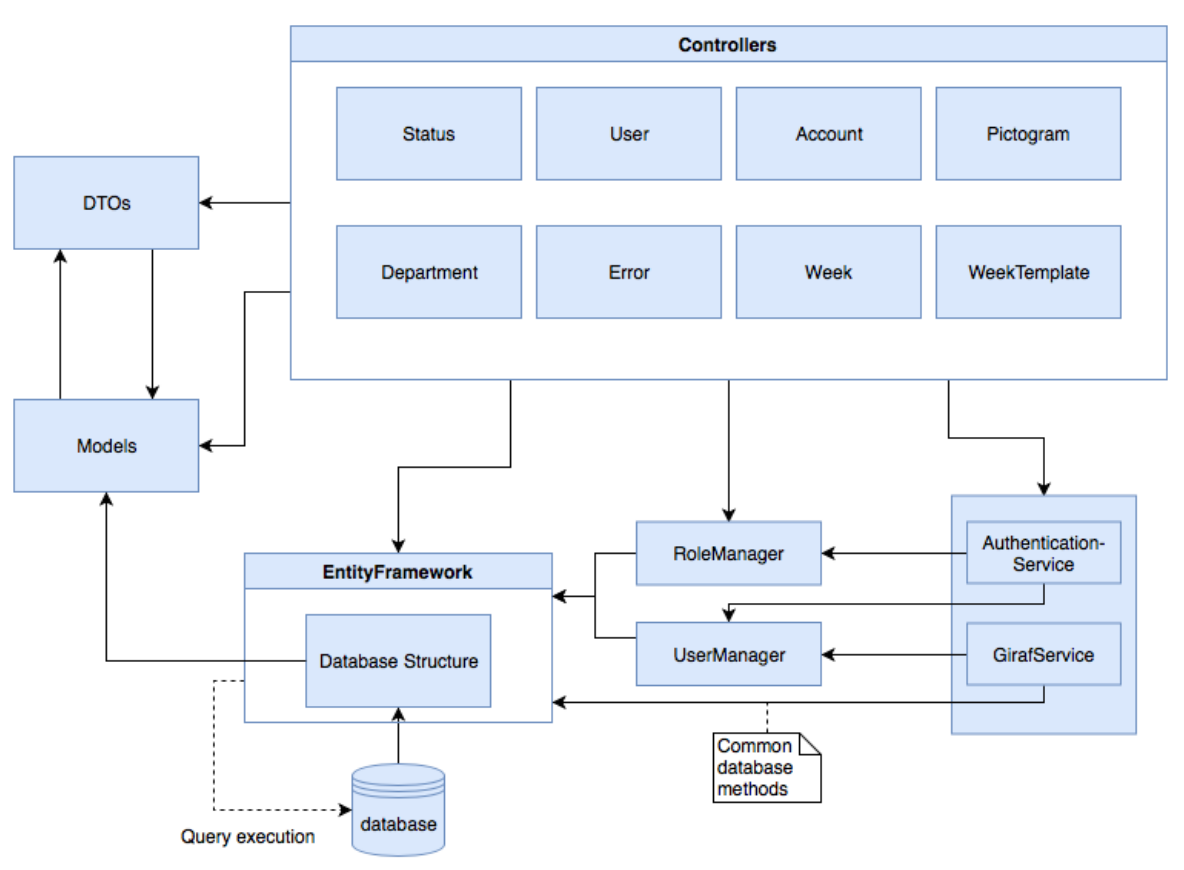
\includegraphics[width=1\textwidth]{figures/api_gen_struct_ho.png}
    \label{fig:app:state-at-handoff:backend}
\end{figure}

\section{Database}\label{app:state-at-handoff:db}

An \gls{er} diagram of the database, generated at the time we overtook the project, is shown on \autoref{fig:app:state-at-handoff:db}.

\begin{figure}[ht]
    \centering
    \caption{Diagram of \gls{er} diagram at the time of handoff}
    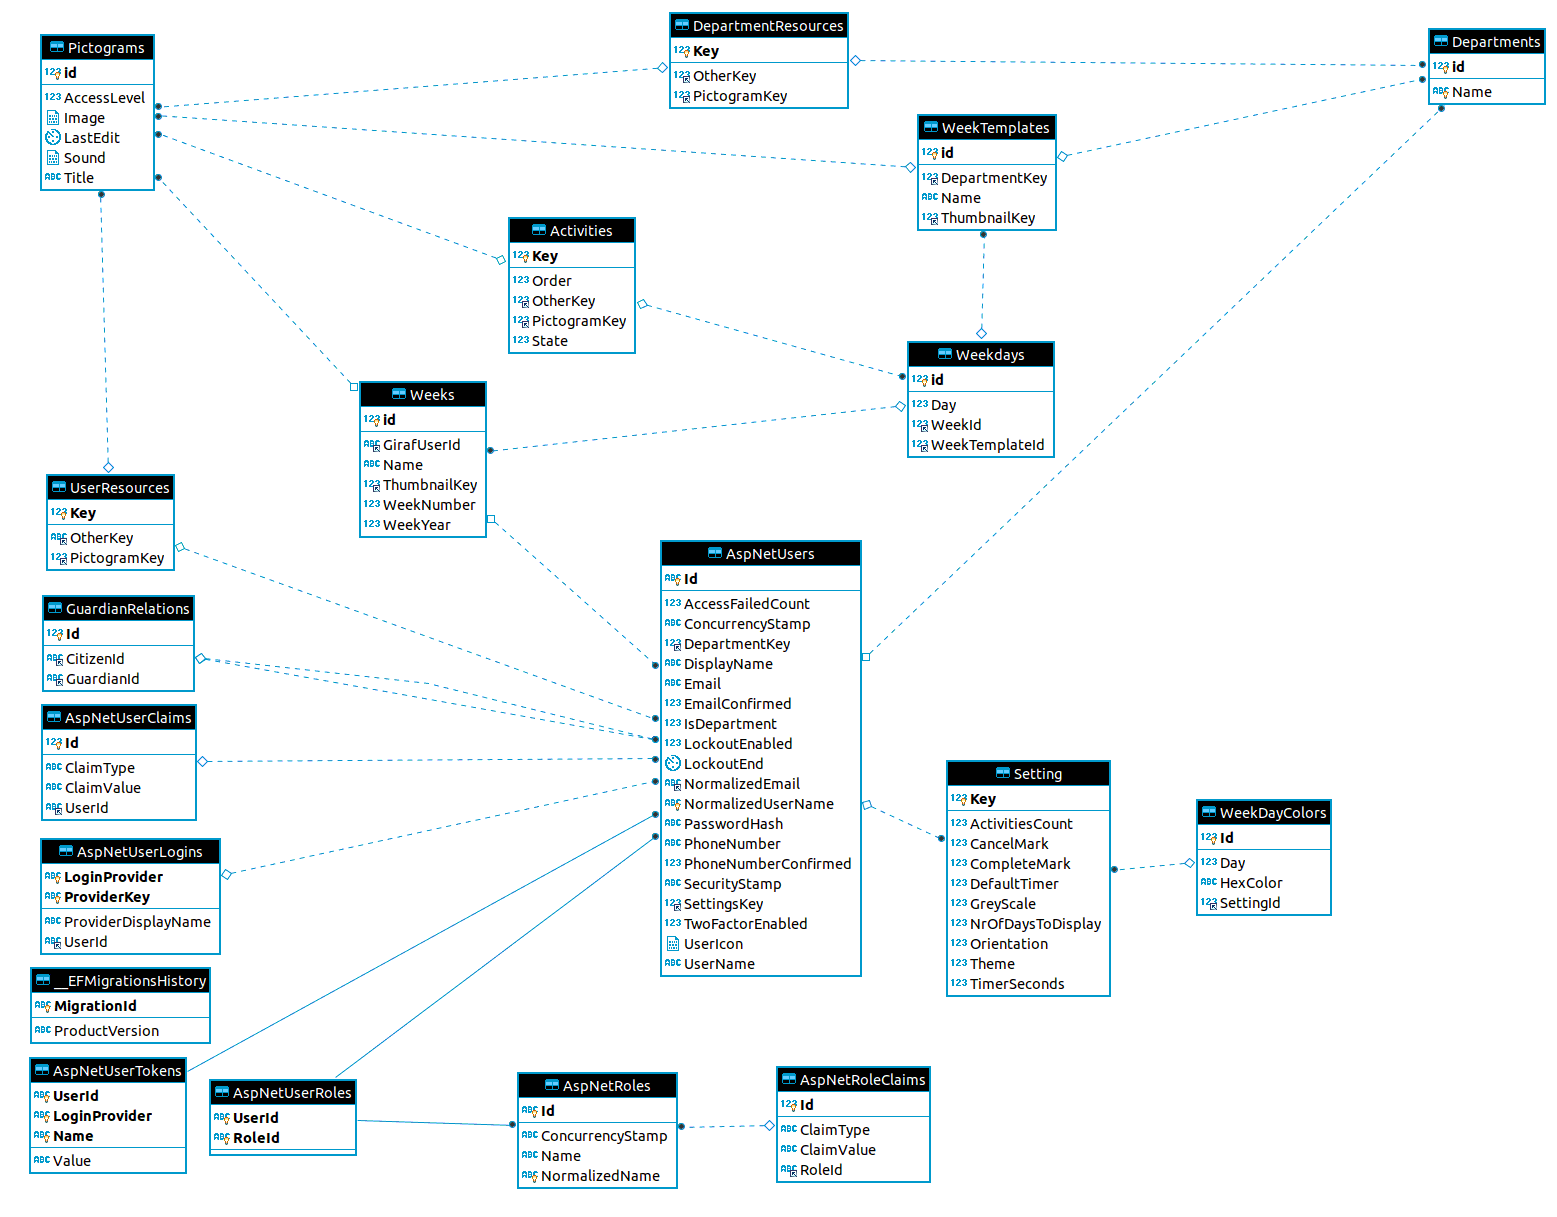
\includegraphics[width=1\textwidth]{figures/db_ho.png}
    \label{fig:app:state-at-handoff:db}
\end{figure}

\section{Endpoints at handoff}\label{app:state-at-handoff:endpoints}

This section describes the different endpoint accessable on the API, at the time of handoff.

\subsection{Account}
For authorizing users these endpoints allow for user login and registering.

\begin{ept}
    \epr{POST}{/v1/Account/login}{This endpoint allows the user to sign in to his/her account by providing valid username and password.}

    \epr{POST}{/v1/Account/register}{Register a new user in the REST-API}

    \epr{PUT}{/v1/User/\{id\}/Account/password}{Allows the user to change his password if they know their old password.}

    \epr{POST}{/v1/User/\{id\}/Account/password}{Allows a user to set a new password if they forgot theirs.}

    \epr{GET}{/v1/User/\{id\}/Account/password-reset-token}{Allows the user to get a password reset token for a given user}

    \epr{DELETE}{/v1/Account/user/\{userId\}}{}

\end{ept}

\subsection{Department}
The endpoints shown below describe how to get and modify information about departments. 

\begin{ept}
    \epr{GET}{/v1/Department}{Get request for getting all the department names.}

    \epr{POST}{/v1/Department}{Create a new department. it's only necesary to supply the departments name}

    \epr{GET}{/v1/Department/\{id\}}{Get the department with the specified id.}

    \epr{GET}{/v1/Department/\{id\}/citizens}{Gets the citizen names.}

    \epr{POST}{/v1/Department/\{departmentId\}/user/\{userId\}}{Add a user that does not have a department to the given department. Requires role Department, Guardian or SuperUser}

    \epr{POST}{\sout{/v1/Department/\{departmentId\}/resource/\{resourceId\}}}{Add a resource to the given department. After this call, the department owns the resource and it is available to all its members.}

    \epr{PUT}{/v1/Department/\{departmentId\}/name}{}

    \epr{DELETE}{/v1/Department/\{departmentId\}}{Endpoint for deleting the GirafRest.Models.Department with the given id}

    \epr{DELETE}{\sout{/v1/Department/resource/\{resourceId\}}}{Removes a resource from the users department.}

\end{ept}

\subsection{Error}
This describes all the error endpoints.

\begin{ept}
    \epr{GET}{/v1/Error}{All Error requests will redirect to this endpoint}

    \epr{PUT}{/v1/Error}{All Error requests will redirect to this endpoint}

    \epr{POST}{/v1/Error}{All Error requests will redirect to this endpoint}

    \epr{DELETE}{/v1/Error}{All Error requests will redirect to this endpoint}

\end{ept}

\subsection{Pictogram}
This describes all the pictogram endpoints.

\begin{ept}
    \epr{GET}{/v1/Pictogram}{Get all public GirafRest.Models.Pictogram pictograms available to the user (i.e the public pictograms and those owned by the user (PRIVATE) and his department (PROTECTED)).}

    \epr{POST}{/v1/Pictogram}{Create a new GirafRest.Models.Pictogram pictogram.}

    \epr{GET}{/v1/Pictogram/\{id\}}{Read the GirafRest.Models.Pictogram pictogram with the specified id id and check if the user is authorized to see it.}

    \epr{PUT}{/v1/Pictogram/\{id\}}{Update info of a GirafRest.Models.Pictogram pictogram.}

    \epr{DELETE}{/v1/Pictogram/\{id\}}{Delete the GirafRest.Models.Pictogram pictogram with the specified id.}

    \epr{GET}{/v1/Pictogram/\{id\}/image}{Read the image of a given pictogram as a sequence of bytes.}

    \epr{PUT}{/v1/Pictogram/\{id\}/image}{Update the image of a GirafRest.Models.Pictogram pictogram with the given Id.}

    \epr{GET}{/v1/Pictogram/\{id\}/image/raw}{Reads the raw pictogram image. You are allowed to read all public pictograms aswell as your own pictograms or any pictograms shared within the department}

\end{ept}

\subsection{Status}
This describes all the status endpoints.

\begin{ept}
    \epr{GET}{/v1/Status}{End-point for checking if the API is running}

    \epr{GET}{/v1/Status/database}{End-point for checking connection to the database}

    \epr{GET}{/v1/Status/version-info}{Endpoint for getting git version info i.e. branch and commithash}

\end{ept}

\subsection{User}
This describes all the user endpoints.

\begin{ept}
    \epr{GET}{/v1/User}{Find information about the currently authenticated user.}

    \epr{GET}{/v1/User/\{id\}}{Find information on the user with the username supplied as a url query parameter or the current user.}

    \epr{PUT}{/v1/User/\{id\}}{Updates the user with the information in GirafRest.Models.DTOs.GirafUserDTO}

    \epr{GET}{/v1/User/\{id\}/settings}{Get user-settings for the user with the specified Id}

    \epr{PUT}{/v1/User/\{id\}/settings}{Updates the user settings for the user with the provided id}

    \epr{GET}{/v1/User/\{id\}/icon}{Endpoint for getting the UserIcon for a specific User}

    \epr{PUT}{/v1/User/\{id\}/icon}{Sets the user icon of the given user}

    \epr{DELETE}{/v1/User/\{id\}/icon}{Deletes the user icon for a given user}

    \epr{GET}{/v1/User/\{id\}/icon/raw}{Gets the raw user icon for a given user}

    \epr{POST}{\sout{/v1/User/\{id\}/resource}}{Add a ressource to another user that the currently authorised user already owns}

    \epr{DELETE}{\sout{/v1/User/\{id\}/resource}}{Deletes the resource of the user with the given Id}

    \epr{GET}{/v1/User/\{id\}/citizens}{Gets the citizens of the user with the provided id. The provided user must be a guardian}

    \epr{GET}{/v1/User/\{id\}/guardians}{Gets the guardians for the specific citizen corresponding to the provided id.}

    \epr{POST}{/v1/User/\{id\}/citizens/\{citizenId\}}{Adds relation between the authenticated user (guardian) and an existing citizen.}

\end{ept}

\subsection{Week}
This describes all the week endpoints.

\begin{ept}
    \epr{GET}{/v1/User/\{userId\}/week}{}

    \epr{GET}{/v1/User/\{userId\}/week/\{weekYear\}/\{weekNumber\}}{Gets the GirafRest.Models.DTOs.WeekDTO with the specified week number and year for the user with the given id}

    \epr{PUT}{/v1/User/\{userId\}/week/\{weekYear\}/\{weekNumber\}}{Updates the entire information of the week with the given year and week number.}

    \epr{DELETE}{/v1/User/\{userId\}/week/\{weekYear\}/\{weekNumber\}}{Deletes all information for the entire week with the given year and week number.}

\end{ept}

\subsection{Weekly Templates}
This describes all the weekly template endpoints.

\begin{ept}
    \epr{GET}{/v1/WeekTemplate}{Gets all schedule templates for the currently authenticated user. Available to all users.}

    \epr{POST}{/v1/WeekTemplate}{Creates new week template in the department of the given user. Available to Supers, Departments and Guardians.}

    \epr{GET}{/v1/WeekTemplate/\{id\}}{Gets the week template with the specified id. Available to all users.}

    \epr{PUT}{/v1/WeekTemplate/\{id\}}{Overwrite the information of a week template. Available to all Supers, and to Departments and Guardians of the same department as the template.}

    \epr{DELETE}{/v1/WeekTemplate/\{id\}}{Deletes the template of the given ID. Available to all Supers, and to Departments and Guardians of the same department as the template.}

\end{ept}

\section{Server}\label{app:state-at-handoff:server}

The server setup is containerized, using docker, as much as possible. Last year they started the transition of making the containers running in a cluster. For this they used Kubernetes. At the point of handoff, only the Gitlab workers run as pots inside Kubernetes.

The Kubeneters is setup with one master node and three other nodes. Besides that, there are three non-clustered servers. \autoref{fig:app:state-at-handoff:server} shows the complete overview of the servers and which services they run.

The server hosting it self is handled by the Aalborg University IT Service Department, where every server is a virtualization using vSphere.

\begin{figure}[h]
    \centering
    \caption{Diagram of the server setup at the time of handoff}
    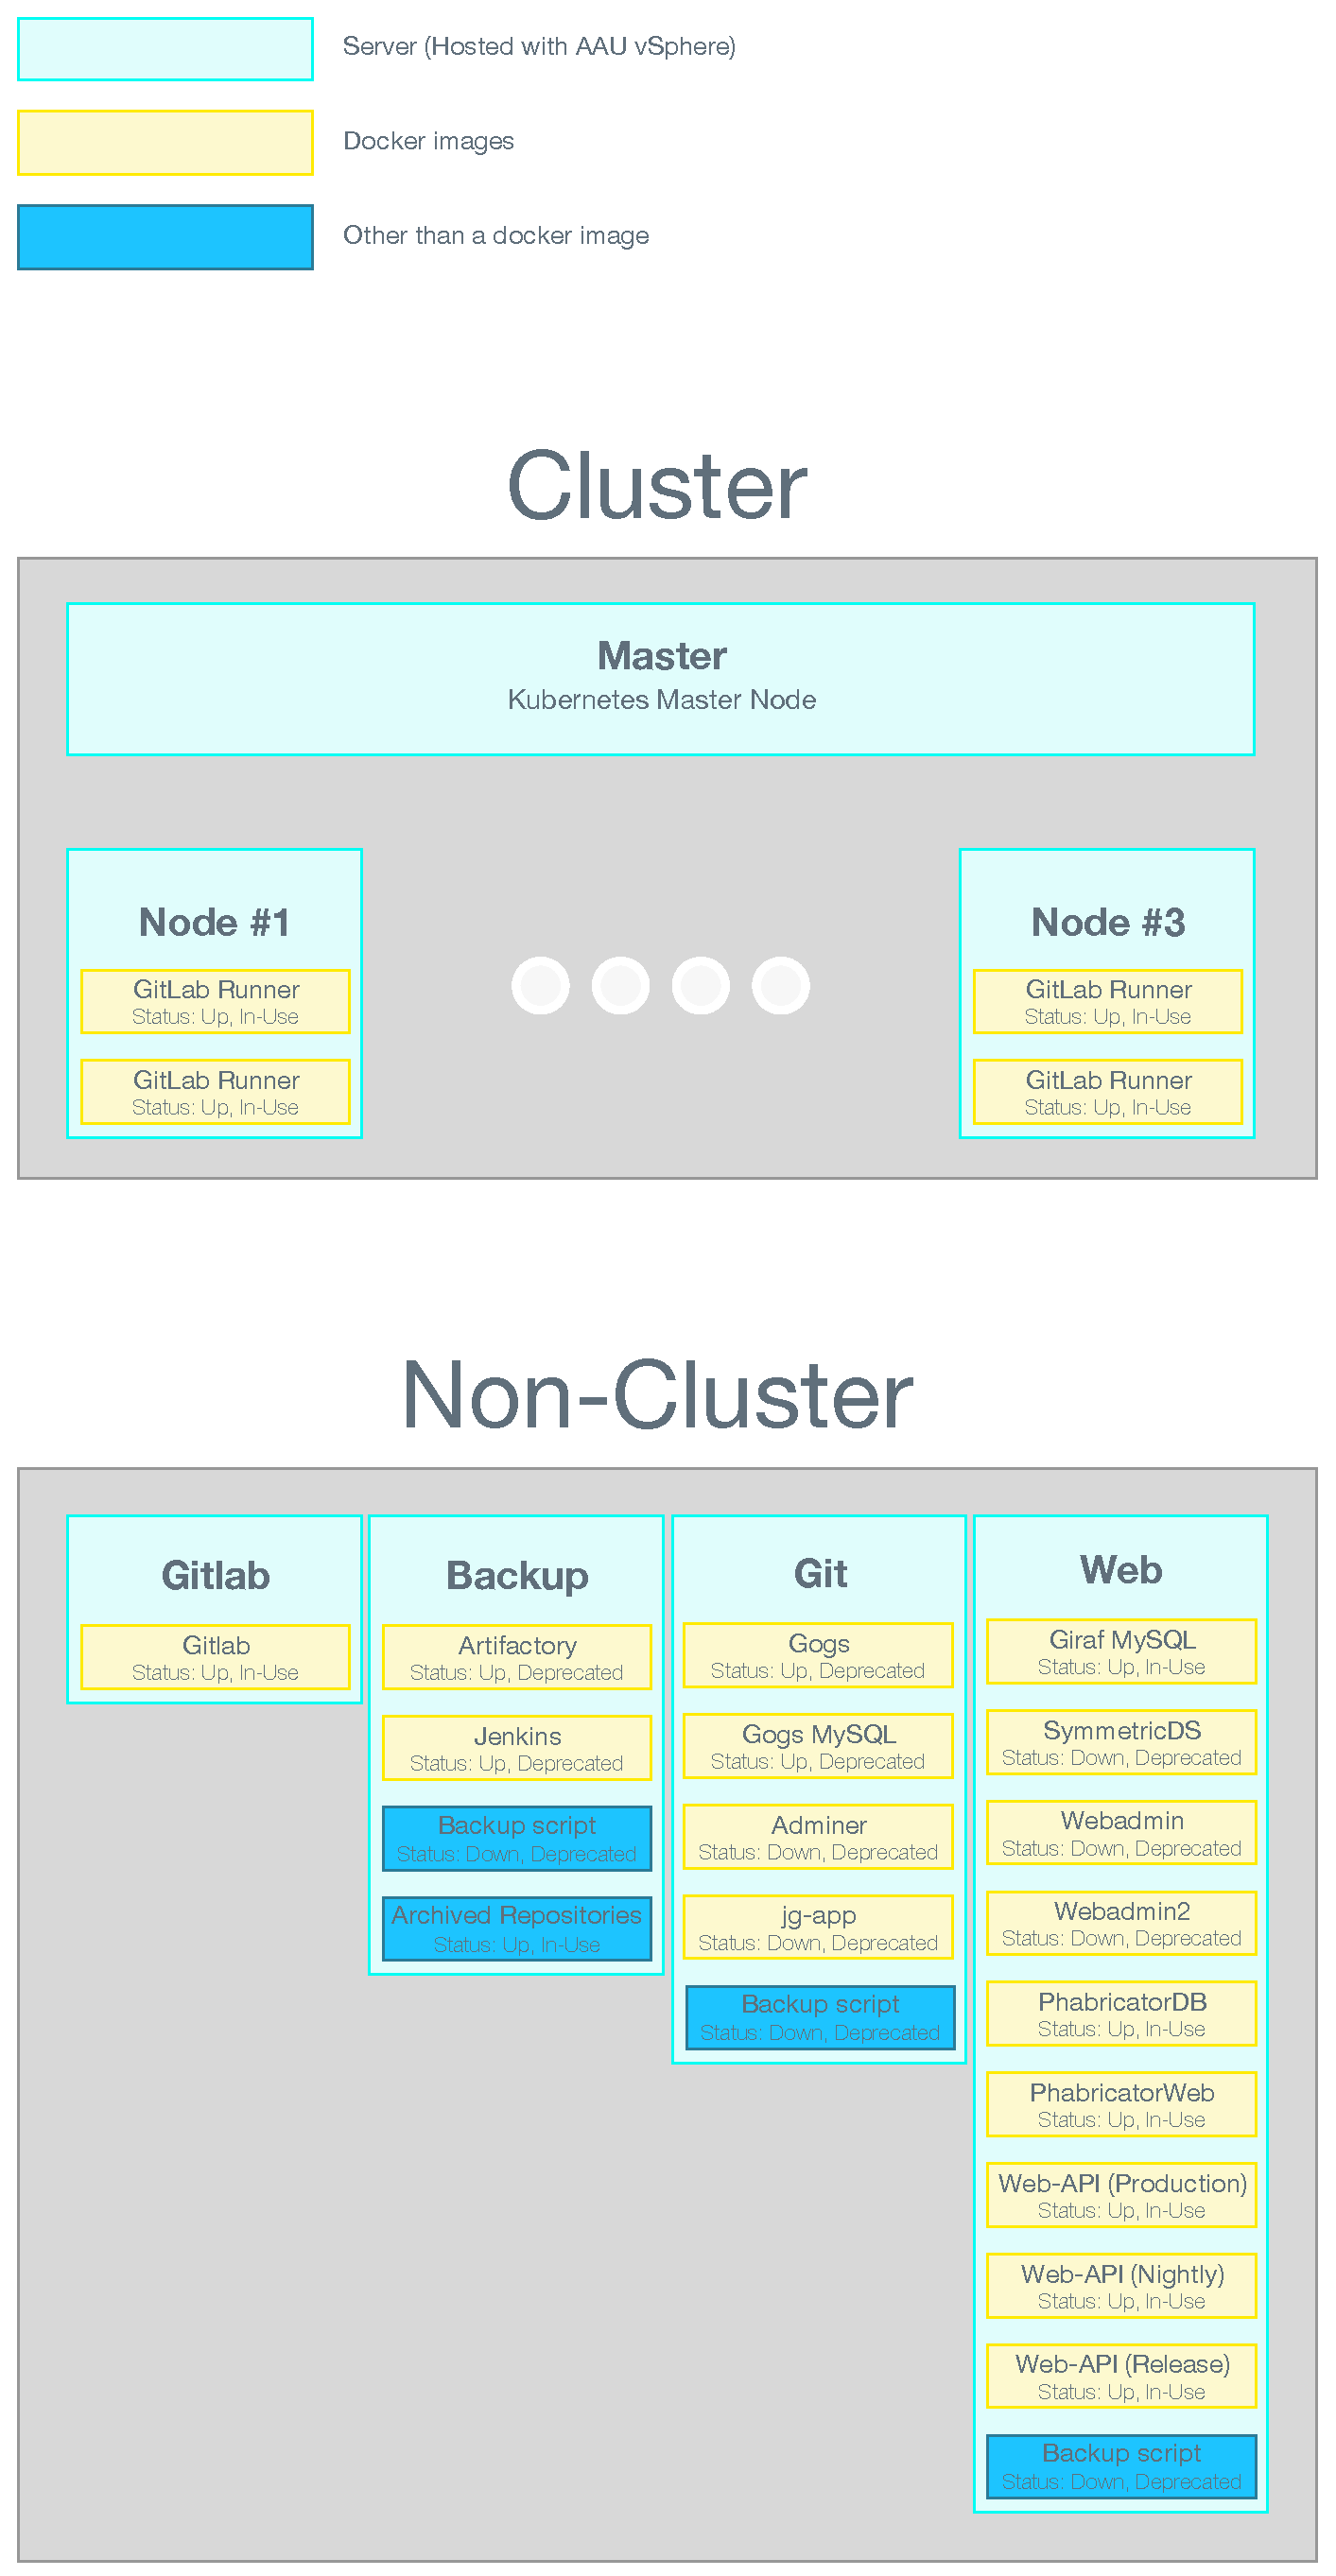
\includegraphics[height=1\textheight]{figures/Server-Overview.pdf}
    \label{fig:app:state-at-handoff:server}
\end{figure}

\chapter{Xamarin Linux Guide} \label{app:xamarin-linux}

\textbf{TODO}: ensure congruency between manual setup and install script

This documents outlines how to setup your environment such that you can
compile the \href{https://github.com/aau-giraf/weekplanner}{WeekPlanner}
app. To compile, you have four different options:

\begin{itemize}
    \item Using a Virtual Machine,
    \item using Docker,
    \item setting it up, manually,
    \item or using the install script.
\end{itemize}

Each of these options will be discussed in the following sections.

\section{Virtual Machine}

To make things easy for everyone, a Virtual Machine is provided. It is
not recommended to use it if not necessary, as it is usually much slower
to do so. But in case you need to, you can download it
\href{https://drive.google.com/file/d/1fxhboUHWcESF-H_CMSkNJFypwQi8fvjI/view?usp=sharing}{here}.
Below are the credentials to the machine.

\begin{lstlisting}
username: aau
password: giraf
\end{lstlisting}

\section{Docker}

Just as the Virtual Machine, the Docker image comes preinstalled with
all the necessary dependancies to compile the project. Of course, to use
Docker you must first ensure that you have installed it. Given that you
have already installed Docker, \lstinline{cd} into your
project directory root, and execute the following, and a brand-new APK
file will appear.

\begin{lstlisting}[language=bash]
docker run -v "$(pwd):/weekplanner" -it aaugiraf/xamarin-android
\end{lstlisting}

If you want to ``ssh'' into the machine, you can attach to the
container's shell by executing the following:

\begin{lstlisting}[language=bash]
docker run -v "$(pwd):/weekplanner" -it aaugiraf/xamarin-android /bin/bash
\end{lstlisting}

For more information regarding the container, look
\href{https://cloud.docker.com/u/aaugiraf/repository/docker/aaugiraf/xamarin-android/general}{here}.

\section{Manually Setup}

To get started we first need root access, this is achieved by running:

\begin{lstlisting}[language=bash]
$ sudo su
\end{lstlisting}

Next, we choose which versions of the different things we're going to
use. We define the following variables for easy reference.

\begin{lstlisting}[language=bash]
DOTNET_SDK_VERSION=2.1.200
XAMARIN_VERSION=8.3.99.189
ANDROID_SDK_TOOLS_VERSION=3859397
\end{lstlisting}

Following this, we will install the general dependencies for Giraf's
Weekplanner.

\begin{lstlisting}[language=bash]
$ apt-get update
$ apt-get -y install \
             unzip \
             openjdk-8-jdk \ # only necessary if not already installed
             libzip4 \
             apt-transport-https \
             curl \
             gnupg
\end{lstlisting}

\subsection{Install Mono}

Installing mono requires adding to the sources list, this is done in the
following bash code:

\begin{lstlisting}[language=bash]
$ apt-key adv --keyserver hkp://keyserver.ubuntu.com:80 --recv-keys 3FA7E0328081BFF6A14DA29AA6A19B38D3D831EF
$ echo "deb https://download.mono-project.com/repo/ubuntu stable-bionic main" | tee /etc/apt/sources.list.d/mono-official-stable.list
$ apt-get update
$ apt-get install -y mono-devel
\end{lstlisting}

\subsection{Installing Android SDK}

To compile to Android, we need the Android SDK. The following will
download the SDK tools and SDK manager.

\begin{lstlisting}[language=bash]
$ curl https://dl.google.com/android/repository/sdk-tools-linux-${ANDROID_SDK_TOOLS_VERSION}.zip -o sdk-tools.zip
$ mkdir /android
$ unzip sdk-tools.zip -d /android
$ rm -rf sdk-tools.zip
$ rm -rf /android/licenses
\end{lstlisting}

We need to agree to some licenses, the following will update the Android
SDK manager, and agree to any licenses.

\begin{lstlisting}[language=bash]
$ yes | /android/tools/bin/sdkmanager --update --licenses
$ yes | /android/tools/bin/sdkmanager "platforms;android-26" "build-tools;27.0.3"
$ yes | /android/tools/bin/sdkmanager --update
\end{lstlisting}

Finally, we fetch the NDK-bundle and change the permission of the
\lstinline{/android/} directory to something more
accessable.

\begin{lstlisting}[language=bash]
$ /android/tools/bin/sdkmanager "ndk-bundle"
$ chmod -R 777 /android/
\end{lstlisting}

\subsection{Installing Xamarin}

Next, we need Xamarin.Android, which can be fetched directly from
Microsoft.

\begin{lstlisting}[language=bash]
$ curl https://xamjenkinsartifact.blob.core.windows.net/xamarin-android/xamarin-android/xamarin.android-oss_${XAMARIN_VERSION}.orig.tar.bz2 -o xamarin.tar.bz2
$ tar xvjf xamarin.tar.bz2
$ mv xamarin.android-oss_* /android/xamarin
$ rm -rf xamarin.tar.bz2
\end{lstlisting}

\subsection{Installing DotNet}

\begin{lstlisting}[language=bash]
$ curl https://packages.microsoft.com/keys/microsoft.asc | gpg --dearmor > microsoft.gpg
$ mv microsoft.gpg /etc/apt/trusted.gpg.d/microsoft.gpg
$ sh -c 'echo "deb [arch=amd64] https://packages.microsoft.com/repos/microsoft-ubuntu-bionic-prod bionic main" > /etc/apt/sources.list.d/dotnetdev.list'
$ apt-get update
$ apt-get install -y dotnet-sdk-${DOTNET_SDK_VERSION}
\end{lstlisting}

\begin{lstlisting}[language=bash]
$ curl https://dist.nuget.org/win-x86-commandline/latest/nuget.exe -o /nuget.exe
$ cp -r /android/xamarin/bin/Release/lib/xamarin.android/* /usr/lib/mono/
$ mkdir -p /usr/lib/mono/xamarin-android/bin/
$ cp -r /android/xamarin/bin/Release/lib/xamarin.android/xbuild/* /usr/share/dotnet/sdk/${DOTNET_SDK_VERSION}
\end{lstlisting}

\subsection{Full script}

The below script was tested on a blank installation of Ubuntu 18.04.2,
and ran successfully.

\begin{lstlisting}[language=bash]
#!/bin/bash
if [ "$EUID" -ne 0 ]
  then echo "Please run as root"
  exit 1
fi

DOTNET_SDK_VERSION=2.1.200
XAMARIN_VERSION=8.3.99.189
ANDROID_SDK_TOOLS_VERSION=3859397

apt-get update
apt-get -y install unzip openjdk-8-jdk libzip4 apt-transport-https curl gnupg

# Set default java version to Java 8
update-java-alternatives --set java-1.8.0-openjdk-amd64

# Ignore saying yes to stuff
DEBIAN_FRONTEND=noninteractive

# Mono
apt-key adv --keyserver hkp://keyserver.ubuntu.com:80 --recv-keys 3FA7E0328081BFF6A14DA29AA6A19B38D3D831EF
echo "deb https://download.mono-project.com/repo/ubuntu stable-bionic main" | tee /etc/apt/sources.list.d/mono-official-stable.list
apt-get update
apt-get install -y mono-devel mono-complete

# Android
curl https://dl.google.com/android/repository/sdk-tools-linux-${ANDROID_SDK_TOOLS_VERSION}.zip -o sdk-tools.zip
mkdir /android
unzip sdk-tools.zip -d /android
rm -rf sdk-tools.zip
rm -rf /android/licenses
yes | /android/tools/bin/sdkmanager --update --licenses
yes | /android/tools/bin/sdkmanager "platforms;android-26" "build-tools;27.0.3"
yes | /android/tools/bin/sdkmanager --update
/android/tools/bin/sdkmanager "ndk-bundle"
chmod -R 777 /android/

# Xamarin
curl https://xamjenkinsartifact.blob.core.windows.net/xamarin-android/xamarin-android/xamarin.android-oss_${XAMARIN_VERSION}.orig.tar.bz2 -o xamarin.tar.bz2
tar xvjf xamarin.tar.bz2
mv xamarin.android-oss_* /android/xamarin
rm -rf xamarin.tar.bz2

# Dotnet
curl https://packages.microsoft.com/keys/microsoft.asc | gpg --dearmor > microsoft.gpg
mv microsoft.gpg /etc/apt/trusted.gpg.d/microsoft.gpg
sh -c 'echo "deb [arch=amd64] https://packages.microsoft.com/repos/microsoft-ubuntu-bionic-prod bionic main" > /etc/apt/sources.list.d/dotnetdev.list'
apt-get update
apt-get install -y dotnet-sdk-${DOTNET_SDK_VERSION}

printf "\nexport ANDROID_SDK_PATH=/android/" >> /etc/environment
printf "\nexport DOTNET_CLI_TELEMETRY_OPTOUT=1" >> /etc/environment
printf "\nexport MSBuildSDKsPath=/usr/share/dotnet/sdk/${DOTNET_SDK_VERSION}" >> /etc/environment

curl https://dist.nuget.org/win-x86-commandline/latest/nuget.exe -o /nuget.exe
cp -r /android/xamarin/bin/Release/lib/xamarin.android/* /usr/lib/mono/
mkdir -p /usr/lib/mono/xamarin-android/bin/
cp -r /android/xamarin/bin/Release/lib/xamarin.android/xbuild/* /usr/share/dotnet/sdk/${DOTNET_SDK_VERSION}
\end{lstlisting}

\section{Common problems}

\subsection{Error \#1}

\begin{lstlisting}[language=bash]
System.TypeInitializationException: The type initializer for 'System.Console' threw an exception. ---> System.TypeInitializationException: The type initializer for 'System.ConsoleDriver' threw an exception. ---> System.Exception: Magic number is wrong: 542
\end{lstlisting}

\begin{lstlisting}[language=bash]
TERM=xterm
\end{lstlisting}

\subsection{Error \#2}

NET Framework 4.5

\begin{lstlisting}
printf "\nexport FrameworkPathOverride=/usr/lib/mono/4.5/" >> /etc/environment
\end{lstlisting}


\chapter{Xamarin Problems} \label{app:xamarin-probelms}

This document will describe why a switch of framework should be considered, and what work lies ahead if a switch is chosen. Keep in mind, that the author's bias towards switching.

\section{Problems with current solution}

Right of the bat, I assume that most of the readers, who run Linux, started by following JetBrain's \href{https://rider-support.jetbrains.com/hc/en-us/articles/360000557259}{How to develop Xamarin.Android applications on Linux with Rider} guide, and were dissapointed to learn that this guide does not lead to a successful compilation of the WeekPlanner app. And as can also be learned by said guide:

\begin{quote}
    Please note that Xamarin.Android on Linux is officially unsupported
\end{quote}

This unfortunate fact, means that approximately a quarter of the developers cannot get started developing without additional hassle.

Without looking at alternative solutions, but using the \href{https://github.com/aau-giraf/xamarin-android/blob/master/Dockerfile}{Dockerfile}, created from last-semester's Docker Image, the following problems were
identified.

\begin{itemize}
    \item Old version of DotNetCore
    \item Non-obvious Xamarin.Android download
    \item Non-standard installation nuget
    \item Complex folder moving and copying
\end{itemize}

It should be noted, that one \emph{can} get compilation to work on
Linux, albeit a hassle. Additional problems occur thereafter, when the
developer tries to compile the Web-Api which no longer works. Following
last-semester's implementation, Linux users, must choose if they want
Web-Api or WeekPlanner to compile.

It should again be noted that one \emph{can} get compilation of the
application and Web-Api to work, by using an IDE that supports multiple
DotNetCore versions.

In my opinion, there are too many loops to go through to achieve an
environment that can compile everything, and if we are to ease the pain
of the comming semester something needs to be done.

\subsection{Additional Problems}

A newly discovered issue lies within the generated code
\href{https://github.com/aau-giraf/weekplanner/tree/master/IO.Swagger}{IO.Swagger}.
IO.Swagger works when downloaded from the repository, but in trying to
regenereate IO.Swagger from a specification file, or from
\texttt{update\_swagger.sh}, results in multiple errors. These errors
are tightly coupled with the Weekplanner project, and as so, are
probably easy fixes.

\section{Solutions}

Some effort has been put in creating an install script (see
\href{https://hackmd.io/_gtHEeO6Q36ww-oANJrJaw}{this}), which can be
extended to get Web-Api to also work. The downside of this solution, is
that the script needs to be maintained, and updating it \emph{might}
result in someone needing to reinstall his/hers OS inorder to get it to
work.

Alternatively, a Dockerised solution can be used, but this solution has
to be created, and set up in a way, that makes compilation, debugging,
and deployment as easy as with other OSes. I personally don't see this
being done in the near future, as this aswell requires major work.

Finally, the nuclear option, switch framework. If we were to switch to
an alternative framework, which supports Windows, MacOS, and Linux, then
everyone will be happy, and there should be no reasonable reason for
future semesters to switch.

\section{Advantages to switching}

There are also many minor advantages of switching, i.e live reloading,
but constraining it to the crux of the problem, the following advantages
were found.

The main issue, that is to be solved by switching framework, is
cross-platform support. It should not be a hassle for any contributor to
get started. In switching to \href{https://flutter.dev/}{Flutter}, this
can be achieved.

Contrary to the current tests, of which there are few, and even fewer
that work, Flutter comes packaged with a testing environment.

Flutter also allows for fixing the fundamental error in the current
structure, of using generated code. The error does not lie in using
generated code, as this can be great when done right, but in the trust
that the generator, or the format it understands, will be supported for
the comming semesters.

\section{Disadvantages to switching}

The biggest disadvantage is reimplentation, as all current code needs to
be ported. Fortunately, this is not too much.

Another disadvantage, if Flutter is chosen as the alternative, is the
paradigm of Flutter. Flutter is OOP but relies on the understanding of
state- or state-less widgets.

Regarding architecture support of Flutter,
\href{https://github.com/flutter/flutter/issues/14925}{it does not
support 32 bit}, which might be a problem, for people with very old
computers.

\section{FAQ}

\begin{quote}
Why not just switch to Windows?
\end{quote}

There are two parts to this answer: 1. Due to the question, I assume
that you run Windows. Would you think it is fair to ask of me in an
alternate setting to switch to Linux? 2. There are many different
reasons people run Linux, one of them is because of Hardware. Not all
computers \textbf{can} run Windows.

\begin{quote}
If we choose to switch, then a LOT of work will go to re-implement
something that already is done. Isn't this a major waste of time?
\end{quote}

There are two sides to this answer. Currently, the app is shit. There is
MAJOR work ahead, to even just get it stable. It is fortunate that the
functionality of the app is very limited, so it is not unreasonable that
the rewrite can be done in a timely manner.

\begin{quote}
But if it \emph{can} work on Linux, why then change?
\end{quote}

The point is not that it cannot be made to work, the point is how many
hoops we have to jump through in order to get it to work. Not everyone
running Linux is a super-nerd that is comfortable playing around with
the terminal and so on. I think it is unreasonable to make them go
through these hoops.

\begin{quote}
Can't the Linux people just work on something else than front-end?
\end{quote}

Yes, but that is not a solution. This excludes 1/4 of the people from
working front-end, which seems really unfair.

\begin{quote}
What about dual-booting Windows?
\end{quote}

By the same argument for why not run Windows full-time, this is not a
viable argument. But also, one might not have disk space to create a
partition for Windows.

\begin{quote}
What is to stop future semesters from switching again, and effectively
nullify our work?
\end{quote}

Look at this way; there are many here who hate C\# and DotNet, but none
of them suggest switching the framework of the Web-Api. That's because
there is no reasonable reason to do so. It is supported on all
platforms, and runs perfectly fine everywhere. The same cannot be said
of the app, but if it were, I believe that by the same reasoning, future
semester would not switch either.

\begin{quote}
If we switch then there is nothing to write about in the report because
everyone needs to work on front-end
\end{quote}

Since our focus this semester was to get the app stable, there should
probably not be too much work in back-end, and server is limited
anyways. And given that there are major problems with the generated
Swagger API, we're in for a major rewrite anyways. Switch or not, I see
most people working in front-end regardless.

\section{Conclusion}

Given the unsupporting nature of Xamarin, a switch is inevitable, it is
only a question of when. I propose ripping the bandaid off, and build a
core, that can be extended by everyone.

\section{Switching}

In case that a switch is decided, then there is some work ahead. To
understand what is to be done, the following two sections will describe
what pages exist currently, and related functionality.

\section{Pages to be implemented}

There are 11/14 pages that need to be re-implemented, in the table
below, the 14 pages are listed and their purpose described.

\begin{longtable}[]{@{}ll@{}}
\toprule
Page name & Description\tabularnewline
\midrule
\endhead
ActivityPage & Info page for Activity\tabularnewline
ChoiceBoardPage ~ & Page for choosing between activities\tabularnewline
ChooseCitizenPage & Vælg Borger\tabularnewline
ChooseTemplatePage & Choose Week Template to use/edit\tabularnewline
CitizenSchedulesPage & Vælg Skema\tabularnewline
CustomNavigationPage & Wrapper to achieve navigation\tabularnewline
LoginPage & Page for logging a user in\tabularnewline
MasterPage & NA\tabularnewline
NewSchedulePage & Tilføj en ny ugepplan\tabularnewline
PictogramSearchPage & Where you search for Pictogram\tabularnewline
SavePromptPage & (Not Used)\tabularnewline
SettingsPage & Page where all settings are listed\tabularnewline
TestingPage & Page for testing views (trivial)\tabularnewline
WeekPlannerPage & Crux of the app, the week overview\tabularnewline
WeekPlannerTemplatePage & Create/Edit Week template\tabularnewline
\bottomrule
\end{longtable}

\section{Other functionality}

\begin{longtable}[]{@{}ll@{}}
\toprule
Category & Description\tabularnewline
\midrule
\endhead
ApplicationObjects & Dependency Injection\tabularnewline
Behaviors & Describe how views can change, e.g select\tabularnewline
Controls & To be used by views\tabularnewline
Converters & To be used by views\tabularnewline
Helpers & Colleciton of functions grouped into classes\tabularnewline
Models & Simple objects that should mainly hold data\tabularnewline
Services & Login, Navigation, Request, and Settings\tabularnewline
Themes & Alternative visible stuff\tabularnewline
Validations & Validation for forms\tabularnewline
ViewModels & Code for the visual stuff\tabularnewline
Views & Visible stuff\tabularnewline
\bottomrule
\end{longtable}

\section{Re-implementation plan}

\begin{itemize}
    \item Core Implementation of the Application in Flutter
    \item Coding standards
\end{itemize}

\end{document}